\begin{frame}

  \frametitle{\textbf{Jet Shapes in HI Collisions}}

  \begin{columns}

    \column{0.4\textwidth}
    \begin{itemize}
    \item The \textbf{jet shape} is the transverse momentum weighted distribution of particles around the jet axis
    \end{itemize}
    \begin{align*}
      \rho(\Delta r) = \cfrac{1}{\delta r} \cfrac{1}{N_{\text{jets}}} \sum_{\text{jets}} \cfrac{\sum_{\text{tracks} \in [r_a, r_b)} p_{\text{T}}^{\text{ch}}}{p_{\text{T}}^{\text{jet}}}
    \end{align*}
    \begin{itemize}
    \item Jets are \textbf{broader} in central collisions
    \item Consistent with picture of a medium-modified parton cascade
    \item Energy is ``pushed out'' of the sides of the jet cone via broadening
    \end{itemize}
    
    \column{0.6\textwidth}

    \centering

    \begin{tikzpicture}
      \node{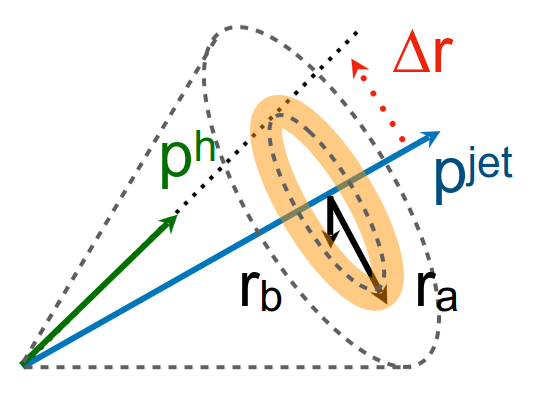
\includegraphics[width=0.5\textwidth]{jet-shape-cartoon.png}};
      \node[font=\tiny] at (1.5,1.6) {\href{https://indico.cern.ch/event/838105/contributions/3519117/attachments/1891832/3120100/HIN-18-020-approval.pdf}{HIN-18-020}};
    \end{tikzpicture}

    \

    \begin{tikzpicture}
      \node{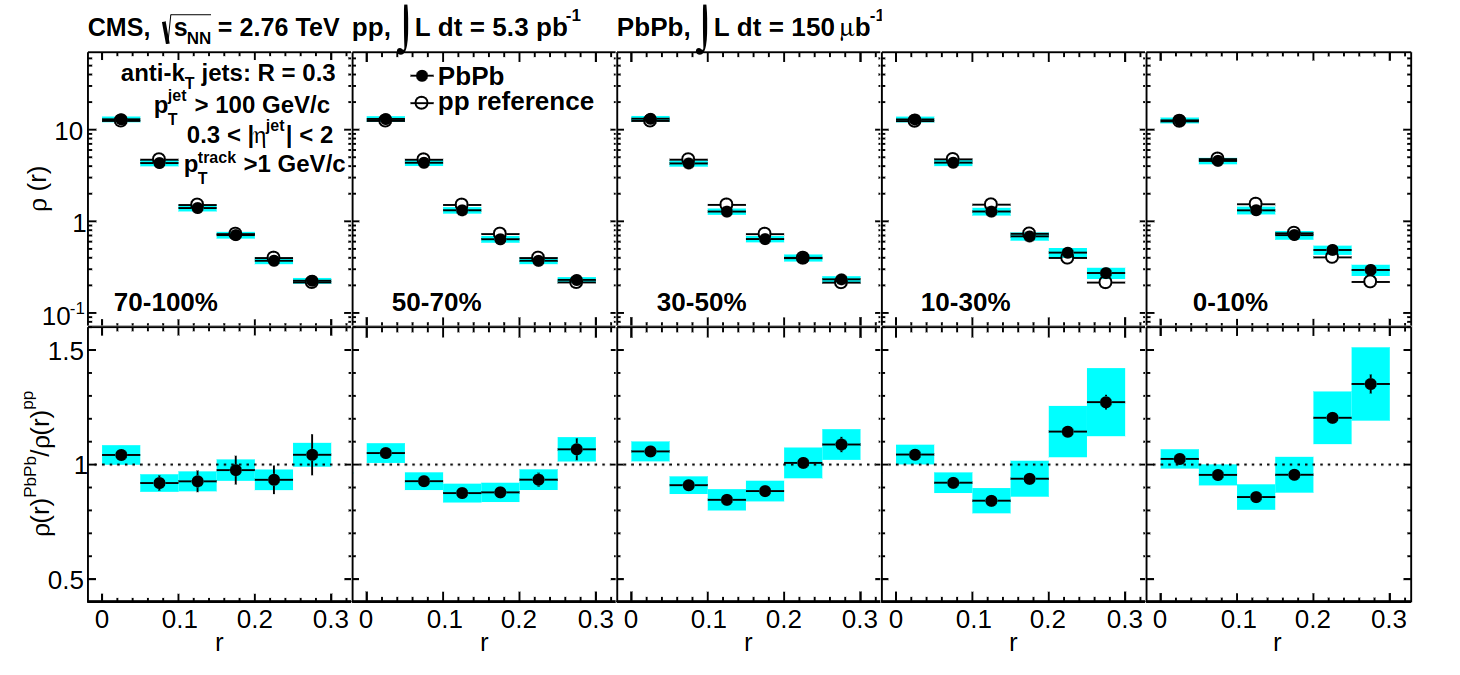
\includegraphics[width=\textwidth]{cms-jet-shape.png}};
      \node[font=\tiny] at (2,1.6) {\href{https://arxiv.org/abs/1102.1957}{arXiv:1102.1957}};
    \end{tikzpicture}


    
    

  \end{columns}






\end{frame}
